\subsection{Qualitätssicherung}

\begin{frame}
  {DECOW14A: Beispiele aus der linguistischen Annotationen}
  \begin{itemize}
    \item 3,866 händische Ergänzungen des TreeTagger-Lexikons
    \item Dependenzparse vom IMS Stuttgart (Sonderversion)

	\vspace{0.5cm}

    \item Named entities mit Stanford Tools + Padó-Modellen

    \begin{itemize}
		\item Genauigkeit evaluiert von Lea Helmers, damals HU\slash FU
		\item Qualität stark abhängig vom Register
		\item Standard: $prec=0.76$ $rec=0.56$
		\item Spontansprachlich: $prec=0.53$ $rec=0.32$
      \end{itemize}
  \end{itemize}
\end{frame}



\begin{frame}
  {DECOW14A: TreeTagger und Mate-Morphology}
  Post-hoc-Evaluation an 10.000 Tokens aus Satzregionen:\\
  TreeTagger exzellent, Mate-Morphology richtig schlecht
  \vspace{0.5cm}
  \begin{center}
    \scalebox{0.8}{
      \begin{tabular}[h]{lrrrrrrrr}
	\hline
	   & POS & Case & Num & Gend & Comp & Per & Tense & Mod \\
	\hline
	\hline
	correct $\approx$ & 0.97 & 0.83 & 0.9 & 0.79 & 0.9 & 0.9 & 0.87 & 0.83 \\
	\hline
      \end{tabular}
    }
  \end{center}

	\begin{itemize}
	  \item Für DECOW16: Marmot-Morphologie,\\SMOR-Pretagging und -Komposita
	\end{itemize}
 
\end{frame}


%\begin{frame}
%	{Evaluation nach Leipziger Art: Satzlängen}
%	\centering
%	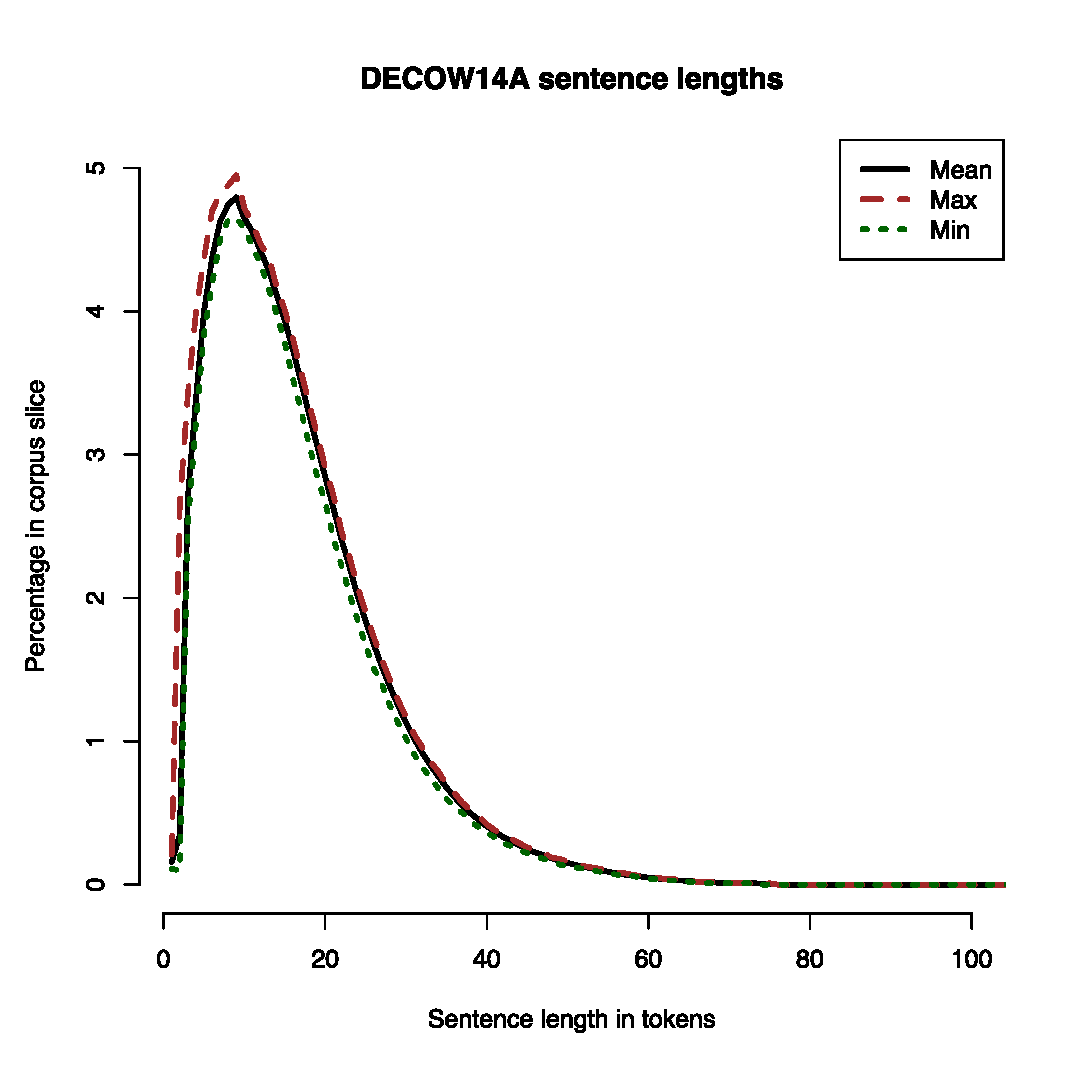
\includegraphics[height=0.8\textheight]{graphics/s_de}
%\end{frame}
%
%\begin{frame}
%	{Evaluation nach Leipziger Art: Satzlängen}
%	\centering
%	\includegraphics[height=0.8\textheight]{graphics/s_en}
%\end{frame}
%
%\begin{frame}
%	{Evaluation nach Leipziger Art: Satzlängen}
%	\centering
%	\includegraphics[height=0.8\textheight]{graphics/s_es}
%\end{frame}
%
%\begin{frame}
%	{Evaluation nach Leipziger Art: Satzlängen}
%	\centering
%	\includegraphics[height=0.8\textheight]{graphics/s_nl}
%\end{frame}
%
%\begin{frame}
%	{Evaluation nach Leipziger Art: Satzlängen}
%	\centering
%	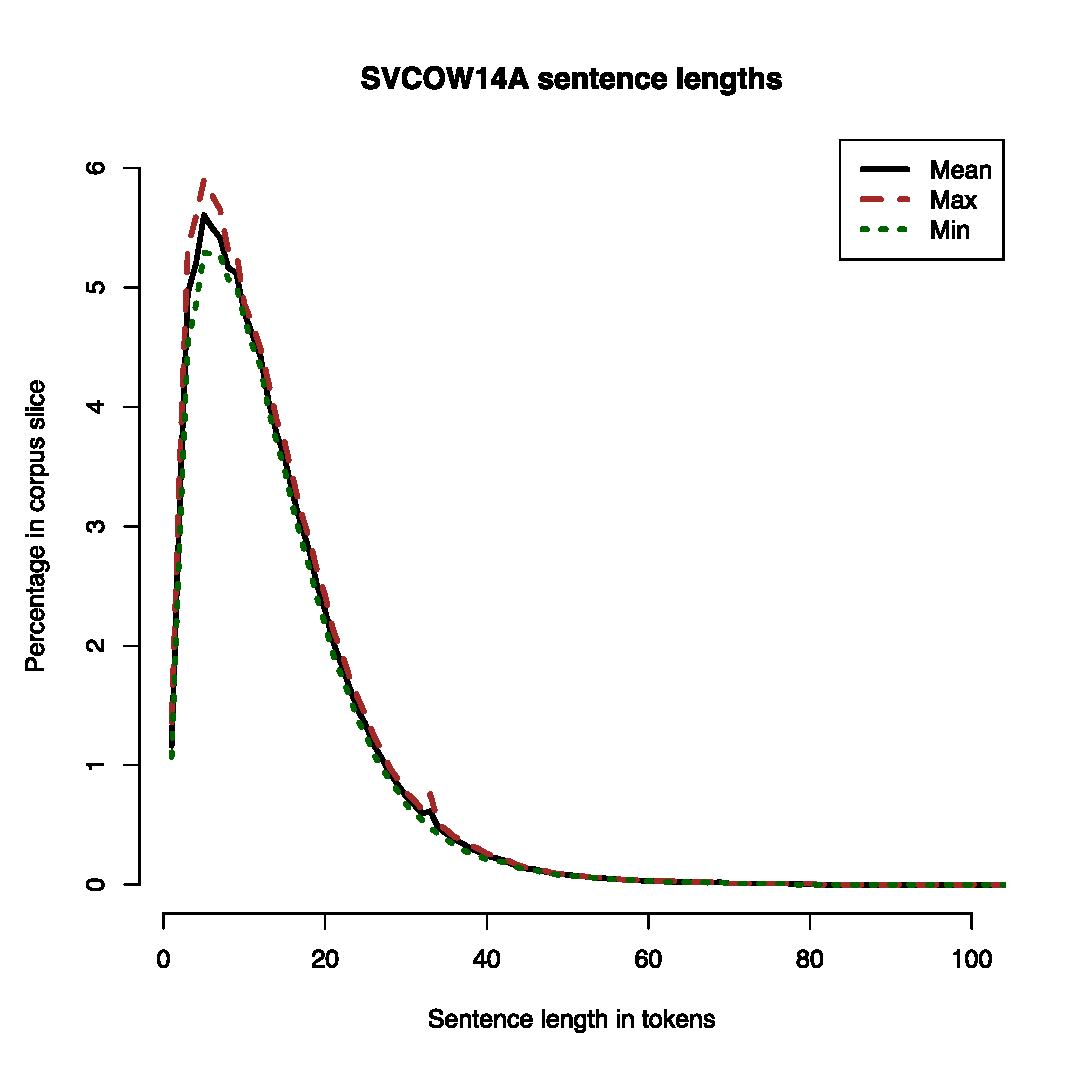
\includegraphics[height=0.8\textheight]{graphics/s_sv}
%\end{frame}

